%%
%% Projeto Oficinas de Integração 3.tex
%% Projeto Oficinas de Integração 3
%% Created by Leonardo Winter Pereira and Lucas Zimmermann Cordeiro on 10.03.2016
%% Copyright (C). All rights reserved
%%

\documentclass[openright]{normas-utf-tex} %openright = O capítulo começa sempre em páginas ímpares
%\documentclass[oneside]{normas-utf-tex} %oneside = Para dissertações com número de páginas menor que 100 (apenas frente da folha)

\usepackage[alf,abnt-emphasize=bf,bibjustif,recuo=0cm, abnt-etal-cite=2]{abntcite} % configuração correta das referências bibliográficas.
\usepackage[brazil, portuges]{babel} % pacote português brasileiro
\usepackage[utf8]{inputenc} % pacote para acentuação direta
\usepackage{amsmath,amsfonts,amssymb} % pacote matemático
\usepackage{graphicx} % pacote gráfico
\usepackage{times} % fonte times
\usepackage{url} % fonte times
\usepackage{listings} % pacote para códigos
\usepackage{pdfsync} % para sincronização automática do PDF
\usepackage{pdfpages} % para poder adicionar documentos PDF ao arquivo
\usepackage{epigraph} % para utilizar epígrafes

%\geometry{left=3.0cm,right=1.5cm,top=4cm,bottom=1cm}       Usado para realizar pequenos ajustes das margens.

% ---------- Preâmbulo ----------
\instituicao{Universidade Tecnológica Federal do Paraná} % nome da instituição
\programa{Bacharelado em Engenharia de Computação} % nome do programa

\documento{Artigo Acadêmico} % [Monografia], [Dissertação] ou [Tese]
\nivel{Graduação} % [Mestrado] ou [Doutorado]
\titulacao{Oficinas de Integração 3} % [Mestre] ou [Doutor]

\titulo{\MakeUppercase{Dalle Pad}} % Título do trabalho em português
\title{\MakeUppercase{Dalle Pad}} % Título do trabalho em inglês

\autor{\hspace{2.25cm}Leonardo Winter Pereira \newline Lucas Zimmermann Cordeiro \hspace{10cm} Luís Felipe Mazzuchetti Ortiz} % Autor do trabalho
\cita{WINTER PEREIRA, Leonardo; ZIMMERMANN CORDEIRO, Lucas; MAZZUCHETTI ORTIZ, Luís F.} % sobrenome (maiúsculas), Nome do autor do trabalho

\palavraschave{Arduino, Android, Projeto, Gerenciamento} % Palavras-chave do trabalho
\keywords{Arduino, Android, Project, Management} % Palavras-chave do trabalho em inglês

\comentario{\UTFPRdocumentodata\ apresentado pelo \UTFPRprogramadata\ da \ABNTinstituicaodata\ como requisito parcial para aprovação na disciplina de "\UTFPRtitulacaodata\ ".}

\orientador{Gustavo Benvenutti Borba \newline Guilherme Alceu Schneider} % nome do orientador do trabalho
\local{Curitiba} % cidade
\data{\the\year} % ano automático

%---------- Inicio do Documento ----------
\begin{document}

    \capa % Geração automática da capa
    \folhaderosto % Geração automática da folha de rosto

    % Dedicatória (Ppcional)
    \begin{dedicatoria}
        AQUI A DEDICATÓRIA
    \end{dedicatoria}

    % Agradecimentos (Opcional)
    \begin{agradecimentos}
        AQUI OS AGRADECIMENTOS
    \end{agradecimentos}

    % Epigrafe (Opcional)
    \begin{epigrafe}
        "A geometria é uma ciência de todas as espécies possíveis de espaços." (Kant)
    \end{epigrafe}

    % Resumo
    \begin{resumo}

        Resumo (Máximo de 500 palavras).

    \end{resumo}

    % Abstract
    \begin{abstract}

        Abstract text (maximum of 500 words).

    \end{abstract}

    % Listas (opcionais, mas recomenda-se a partir de 5 elementos)
    \listadefiguras % Geração automática da lista de figuras
    \listadetabelas % Geração automática da lista de tabelas
    \listadesiglas % Geração automática da lista de siglas
    \listadesimbolos % Geração automática da lista de símbolos

    % Sumário
    \sumario % Geração automática do sumário

    %---------- Início do Texto ----------
    %%
%% Introducao.tex
%% Projeto Oficinas de Integração 3
%% Created by Leonardo Winter Pereira and Lucas Zimmermann Cordeiro on 10.03.2016
%% Copyright (C). All rights reserved
%%

\chapter{Introdução}
\label{chap:introducao}

    \textbf{DALLE PAD - O Gadget que te transforma em um DJ} foi desenvolvido para a disciplina de Oficina de Integração 3 (IF66J - S71), do curso de Engenharia de Computação da Universidade Tecnológica Federal do Paraná.

    Como proposto pela disciplina, o sistema é composto por uma estação base principal (desenvolvida para \textit{Desktop e notebook}) e outra secundária (desenvolvida para \textit{mobile}), um sistema de comunicação e um sistema embarcado. Em ambas as estações base encontram-se os softwares de interface com o usuário; o sistema de comunicação é baseado em tecnologia sem fio, além de conexão \sigla{USB}{Universal Serial Bus} e \sigla{MIDI}{Musical Instrument Digital Interface}; o sistema embarcado consiste em um sistema microcontrolado e a estrutura física do produto é composta por um invólucro mecânico contendo todo o sistema microcontrolado e toda a estrutura física necessária para que o usuário final possa utilizar tudo o que o \textbf{DALLE PAD} permite.

    Este capítulo divide-se em nove seções. Na Seção 1.1 e 1.2, apresentam-se o tema e a delimitação do projeto, respectivamente. Na Seção 1.3, enuncia-se o problema cuja solução é proposta neste trabalho. Na Seção 1.4, enunciam-se os objetivos geral e específicos. A justificativa e o procedimento metodológico adotados s˜ao descritos, respectivamente, nas seções 1.5 e 1.6. Na Seção 1.7 é apresentado o embasamento teórico, na Seção 1.8 é apresentada a estrutura do restante do trabalho e por fim, na Seção 1.9, é apresentada a banca examinadora e pessoas convidadas para a defesa do trabalho.

    \section{Tema}

        A música é a arte de combinar sons de maneira agradável ao ouvido e a sensibilidade emocional utilizando elementos como melodia, harmonia e ritmo. Atualmente, não se conhece nenhuma civilização ou agrupamento que não possua manifestações musicais próprias. A criação, o desempenho, o significado e até mesmo a definição de música variam de acordo com a cultura e o contexto social, como composições fortemente organizadas e improvisadas.

        A música expandiu-se ao longo dos anos, e atualmente encontra-se em diversas utilidades, não só como arte, mas também como a militar, educacional ou terapêutica (musicoterapia). Além disso, tem presença central em diversas atividades coletivas, como os rituais religiosos e festas.~\cite{PPD}

        Os instrumentos musicais até o século XIX baseavam-se em um mesmo princípio de produção sonora, todo som era proveniente da vibração de algum material elástico (as cordas do violão e do piano, por exemplo) que gerava ondas que se propagam pelo ar até atingirem o sistema auditivo do ouvinte. Entretanto, o surgimento de novas tecnologias baseadas na eletricidade e no uso de sinais eletromagnéticos abriu a possibilidade da geração de sons artificiais, sem a utilização de instrumentos mecânicos. Embora as ondas que atingem os ouvidos possuam a mesma natureza, a sua produção é radicalmente diferente.~\cite{SANTINI2005}

        Para alguns indivíduos, a música está extremamente ligada à sua vida, mas a dificuldade de manter um grupo musical unido é muito grande, sem contar o custo elevado de determinados instrumentos e outros equipamentos. Atualmente, pode-se contar com a Tecnologia MIDI.

        Desde seu lançamento no mercado no inicio da década de 1980, o protocolo MIDI tem tido um papel de grande importância na indústria da música. Entretanto, mais importante ainda é que este trouxe para músicos e entusiastas uma ferramenta que lhes permitiu preencher a lacuna antes existente. MIDI permitiu, pela primeira vez, um meio de comunicação de informações musicais de um dispositivo para outro de uma forma que foi aceito e adotado por toda uma indústria.~\cite{Guerin}

        Alguns anos mais tarde, em meados da década de 1990, alguns acreditavam que MIDI não tinha mais futuro. Estações de trabalho de áudio digital foram se tornando cada vez mais acessíveis e computadores passaram a oferecer um poder de processamento cada vez maior, que o uso de MIDI foi quase considerada uma coisa do passado, lento demais para continuar sendo utilizado. Entretanto, não foi isso o que aconteceu.

        Este protocolo continua sendo amplamente utilizado na área musical, e é de interesse deste projeto compreender a teoria por trás do mesmo, não somente sua utilização no produto final, o controlador DALLE PAD.

        Inspirado em diversos produtos já existentes, o protótipo aqui apresentado será capaz de realizar todas as principais funções de um controlador MIDI (a ser explicitado no decorrer deste documento).

    \section{Delimitação do Estudo}

        Este trabalho busca disponibilizar as informações necessárias sobre o protocolo MIDI para os leitores interessados, incluindo sua importância, utilidade e formas de utilização, além de explicar a teoria por trás de todos os conceitos utilizados neste protótipo. Desta forma, até mesmo o leitor leigo na área de computação musical poderá acompanhar este trabalho sem maiores problemas.

        Com o objetivo de desenvolver um produto acessível para o usuário final, procurou-se componentes de baixo custo e interfaces gráficas para trabalhar em conjunto com o mesmo que fossem comuns e de fácil aquisição: computadores, \textit{notebooks}, \textit{smartphones} e \textit{tablets}.

    \section{Problema}

        O trabalho consiste na confecção de um controlador MIDI e sua integração à um sistema através do uso das comunicações \textit{bluetooth}, USB e MIDI. Com o objetivo principal do trabalho sendo adquirir experiência e aprendizado quanto aos elementos envolvidos, o problema do projeto se limita à utilização do \textit{bluetooth} e ao custo total do projeto. Ao longo do desenvolvimento do projeto, o problema que se procura resolver é: Existe como confeccionar um controlador MIDI que utilize as comunicações citadas e que possua custo acessível?

        A primeira etapa do desenvolvimento do projeto se baseia na escolha dos componentes e sua montagem, procurando a solução quanto aos custos totais. Já na segunda fase, o desenvolvimento da integração com um sistema irá permitir avaliar a viabilidade do \textit{bluetooth} no projeto.

    \section{Objetivos}

        Nesta seção são apresentados os objetivos geral e específicos do trabalho, relativos ao problema anteriormente apresentado.

        \subsection{Objetivos Gerais}

            Desenvolver um controlador MIDI capaz de exercer todas as principais funções impostas a ele no meio musical, através de um dispositivo que possua sistema operacional \textit{Android} e comunicação por \textit{bluetooth} ou através de um computador ou \textit{notebook} que possua o sistema operacional \textit{Windows}, utilizando-se das comunicações USB e MIDI.

        \subsection{Objetivos Específicos}

            \begin{itemize}
              \item Estudo profundo do protocolo MIDI;

              \item Projetar e montar o protótipo do controlador aqui proposto;

              \item Desenvolver um aplicativo para \textit{Android} capaz de se comunicar com o mesmo;

              \item Desenvolver um software para \textit{Windows} capaz de trabalhar com arquivos MIDI e de se comunicar com o controlador;

              \item Implementação do protocolo de comunicação entre as estações base e o controlador.
            \end{itemize}

    \section{Justificativa}



    \section{Procedimentos Metodológicos}

        A natureza deste trabalho é de pesquisa aplicada, pois gerará um protótipo de aplicação prática, dirigido a um problema específico. A abordagem é qualitativa, envolvendo testes do projeto em ambiente simulado.

        O seu desenvolvimento é organizado em três principais estágios: pesquisa bibliográfica, implementação e experimentação. Na fase de pesquisa bibliográfica, s˜ao considerados os resultados de trabalhos passados que se mostraram relevantes para a implementação do presente projeto, desde os conceitos mais abrangentes (e.g.: ) até os mecanismos básicos (e.g.: ).

        %TODO

    \section{Embasamento Teórico}

        Para que seja possível a execução deste projeto, diversas referências serão utilizadas.

        Referente ao protocolo MIDI, serão utilizados como referencial teórico, principalmente, ~\cite{Alves}, ~\cite{Hewitt}, ~\cite{Colbeck}, ~\cite{Guerin}, ~\cite{McGuire} e ~\cite{Huber}, mas diversos outros trabalhos serão citados no decorrer deste trabalho.

        Referente às estações base, os principais referenciais teóricos são, além dos já citados anteriormente, ~\cite{Ballou}, ~\cite{Gregoire}, ~\cite{Jackson}, além de ~\cite{AndroidDeveloper}.

        Por último, para o sistema microcontrolado, as principais referencias são ~\cite{Wheat}, ~\cite{Bayle}, ~\cite{Ghassaei} e ~\cite{Hass}, além de ~\cite{Arduino2014}, ~\cite{ArduinoRef2014}.

    \section{Estrutura do Trabalho}

        O trabalho terá a estrutura abaixo apresentada:

        \begin{itemize}
          \item Capítulo 1 - Introdução: são apresentados o tema, as delimitações da pesquisa, o problema e a premissa, os objetivos da pesquisa, a justificativa, os procedimentos metodológicos, as indicações para o embasamento teórico e a estrutura geral do trabalho.

          \item Capítulo 2 - Fundamentação Teórica: são apresentados os conceitos e equipamentos necessários para a construção do Dalle Pad.

          \item Capítulo 3 - Desenvolvimento: é apresentado o funcionamento do Hardware e Software do Dalle Pad, bem como a comunicação entre ambas as partes.

          \item Capítulo 4 - Resultados e Discussões: são apresentados os resultados obtidos e discussões pertinentes.

          \item Capítulo 5 - Considerações Finais: serão retomadas a pergunta de pesquisa e os seus objetivos e apontado como foram solucionados, respondidos, atingidos, por meio do trabalho realizado. Além disto, serão sugeridos trabalhos futuros que poderiam ser realizados a partir do estudo realizado.
        \end{itemize}

    \section {Banca Examinadora}

        Durante toda a execução deste projeto, diversos alunos e professores foram de extrema ajuda e importância.

        É com grande alegria que nomeio alguns destes para participar da banca examinadora do projeto:

    \begin{itemize}
        \item Aluno(s) convidado(s):

            \subitem João Pedro Curti

            \subitem André Eleutério

        \item Professor orientador:

            \subitem César Manuel Vargas Benitez (DAELN)

            \subitem Rafael Barreto (DAFIS)

        \item Professor(a) convidado(a):

            \subitem Leyza Dorini (DAINF)

            \subitem Fábio Dorini (DAMAT)

        \item Professor(es) da disciplina:

            \subitem Gustavo Benvenutti Borba (DAELN)

            \subitem Guilherme Alceu Schneider (DAELN)

    \end{itemize} 
    %%
%% FundamentacaoTeorica.tex
%% Projeto Oficinas de Integração 3
%% Created by Leonardo Winter Pereira and Lucas Zimmermann Cordeiro on 10.03.2016
%% Copyright (C). All rights reserved
%%

\definecolor{darkRed}{rgb}{0.607843137254902, 0.1764705882352941, 0.1215686274509804}
\definecolor{lightRed}{rgb}{0.9568627450980392, 0.803921568627451, 0.7843137254901961}

\newcolumntype{C}[1]{>{\centering\let\newline\\\arraybackslash\hspace{0pt}}m{#1}}


\chapter{Fundamentação Teórica}
\label{chap:fundamentacaoTeorica}

    Para uma melhor compreensão e análise do funcionamento e princípios envolvidos em um controlador MIDI, é fundamental entendermos todos os conceitos nesse processo, bem como as características das tecnologias utilizadas na construção do protótipo e de ambos os aplicativos de controle. Assuntos, esses, que serão tratados no decorrer dessa seção.

    \section{MIDI}

        Uma vez que o projeto aqui proposto baseia-se, basicamente, no funcionamento deste protocolo e na troca de informações deste com outros dispositivos, é imprescindível um completo entendimento do mesmo.

        Esta será a mais longa seção deste capítulo, mas também a mais importante. Além disso, aqui serão citados grandes nomes utilizados como referência para este projeto, para o caso de o leitor se interessar pelos conteúdos aqui expostos e quiser se aprofundar nos mesmos.

        \subsection{O que é MIDI}

            O primeiro conceito que o leitor deve entender é o que é, de fato, o protocolo MIDI, citado repetidas vezes no capítulo anterior, mas que ainda não foi explicitado. Para tanto, serão citadas três definições deste e após, será estudado o real significado das mesmas.

            Adam Olson, do Conservatório Shenandoah, define MIDI como: \epigraph{[...] MIDI é um protocolo de controle que envia dados entre vários instrumentos musicais e sequênciadores.}{~\cite{McGuire}}

            Já David Miles Huber, autor do livro \textit{The MIDI Manual} define MIDI como: \epigraph{[...] Basicamente, MIDI é uma linguagem e especificação compatível de comunicação digital que permite múltiplos hardwares e softwares se comunicarem uns com os outros através de uma rede conectada.}{~\cite{Huber}}

            Robert Guérin, autor do livro \textit{MIDI Power!}, por sua vez, define MIDI como: \epigraph{[...] MIDI permite que músicos, engenheiros de som e iluminação, entusiastas da computação, ou qualquer outra pessoa usem computadores e instrumentos musicais eletrônicos para criar, ouvir e aprender sobre música, oferecendo uma linguagem comum que é compartilhado entre dispositivos e software compatíveis.}{~\cite{Guerin}}

            Com estas definições, pode-se perceber que MIDI é, por si só, incapaz de reproduzir som. Esta é sua maior qualidade. Seus dados podem ser gravados em um programa de software (conhecido como sequênciador) ou dispositivo de hardware, onde estes podem ser editados e transmitidos para instrumentos eletrônicos ou outros dispositivos para criar a música ou controlar qualquer parâmetro desejado. Além disso, MIDI pode ser separado em três entidades diferentes: A linguagem utilizada, também conhecida como protocolo de comunicação; a interface de hardware utilizada para transmitir e receber essas informações (tais como conectores e cabos); e os formatos de distribuição, tal como \sigla{SMF}{Standard MIDI Files} (Arquivos MIDI padrão). No decorrer deste capítulo, abordaremos separadamente cada entidade, a fim de entender como elas trabalham juntas e o porquê do MIDI funcionar tão bem, oferecendo interconectividade, flexibilidade e (em termos de tamanho de arquivo) portabilidade.

            Fundamentalmente, MIDI é uma linguagem de descrição de música em forma binária, em que cada palavra binária descreve um evento de uma música. Cada instrumento musical realiza um som, o qual está totalmente sobre controle do músico. O músico controla o momento em que o instrumento começará a realizar um determinado som - um tecladista pressionará uma tecla, um trompetista soprará ar e um baixista puxará uma corda. Considere esta ação como o evento \textbf{Note ON}. A mensagem MIDI em si não contém o real som tocado pelo instrumento, mas sim a ação de tocar uma determinada nota em um determinado momento e durante um determinado período.

            Quando o músico deixa de pressionar uma tecla em seu teclado ou de puxar uma corda em seu baixo, o som pára. Com MIDI, quando tal ação é realizada, uma mensagem é enviada para essa nota, para que esta deixe de realizar som. Esta mensagem é conhecida por \textbf{Note OFF}. A figura ~\ref{fig:MIDI_Nota_ON_e_OFF} demonstra um exemplo destes dois eventos.

            \begin{figure}[H]
            	\centering
            	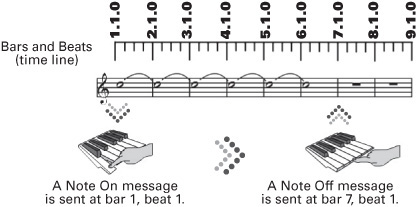
\includegraphics{Imagens/MIDI_Nota_ON_e_OFF.jpg}
            	\caption[Exemplo de transmissão das mensagens de Nota ON e OFF]{Exemplo de transmissão das mensagens de Nota ON e OFF ~\cite{Guerin}}
            	\label{fig:MIDI_Nota_ON_e_OFF}
            \end{figure}

            A fim de identificar qual nota foi ativada / desativada no instrumento, um número é atribuído para cada nota. MIDI também lida com valores interpretativos, como por exemplo a velocidade que a nota foi pressionada e a pressão que é executada na mesma.

        \subsection{O protocolo de comunicação MIDI}

            O protocolo de comunicação MIDI é transmitido de forma serial ao invés de paralela. Em uma transmissão paralela, como o nome sugere, as informações são transmitidas simultaneamente. A quantidade de dados que podem ser transmitidos simultaneamente depende na capacidade física do fio e da velocidade com que os dispositivos podem enviar suas informações. Na figura ~\ref{fig:Parallel_versus_serial_transmissions}, podemos perceber que um \textit{byte} (oito \textit{bits}) é transmitido simultaneamente utilizando uma transmissão paralela. A transmissão serial, por outro lado, consegue enviar apenas um \textit{bit} após o outro.

            \begin{figure}[H]
            	\centering
            	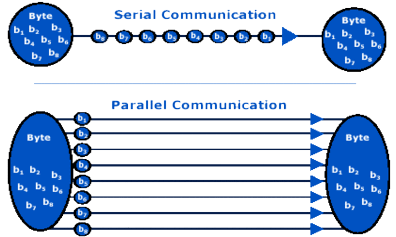
\includegraphics[scale=0.8]{Imagens/Parallel_versus_serial_transmissions.png}
            	\caption[Comparação entre transmissão serial e paralela]{Comparação entre transmissão serial e paralela}
            	\label{fig:Parallel_versus_serial_transmissions}
            \end{figure}

            A pergunta que fica é: Por que MIDI usa transmissão serial ao invés da transmissão paralela?

            A resposta para essa pergunta está no período em que o protocolo foi desenvolvido. A transmissão paralela tinha algumas desvantagens que superavam as vantagens desta sobre a transmissão serial, além de ser muito mais cara, uma vez que os fios, conectores e tomadas eram mais complexos. Já a transmissão serial, por outro lado, era muito mais simples de ser produzida, mais acessível para o público e rápida o suficiente para os fins que os fabricantes e usuários tinham em mente naquela época, para não mencionar mais confiável. Com o passar dos anos, a tecnologia avançou muito e os custos da transmissão paralela despencaram. Entretanto, para manter o MIDI compatível com todos os antigos dispositivos, sua forma de transmissão de dados permaneceu inalterada desde sua introdução no mercado.

            MIDI envia informação a uma taxa de 31250 \sigla{bps}{\textit{bits} por segundo}. Essa velocidade é chamada de taxa de transmissão. Uma vez que o protocolo utiliza transmissão serial, o mesmo envia apenas um \textit{bit} por vez. Cada \textit{byte} em uma mensagem MIDI contém 10 \textit{bits} de dados (8 \textit{bits} para as informações e 2 \textit{bits} para correção de erro). Isso significa que MIDI envia cerca de 3125 \textit{bytes} de dados cada segundo.

            Quando comparamos esse valor com a taxa de transmissão de 176400 \textit{bytes} necessária para transmitir áudio digital (reprodução e gravação) em formado de CD de áudio, MIDI pode parecer incrivelmente devagar. Entretanto, neste último não é necessário enviar tanta informação quanto o áudio digital, sendo capaz de, teoricamente, transmitir até 500 mensagens MIDI por segundo. Na realidade, leva cerca de um milésimo de segundo para transmitir uma única nota. O limiar para distinguir os eventos de som individuais é de aproximadamente 10 milissegundos, então você apresentará dificuldades com 10 ou mais eventos simultâneos.

        \subsection{Hardware e conectores}

            Informações MIDI são transmitidas através de fios e conectores, e seus cabos podem apresentar até 15 metros de comprimento. Entretanto, por se tratar de um cabo serial, todos os dados são transmitidos através de um único fio principal, e grandes distâncias podem inferir em uma degradação do sinal, ocasionando em possíveis perdas de dados ou mensagens impossíveis de serem lidas.

            \begin{figure}[H]
            	\centering
            	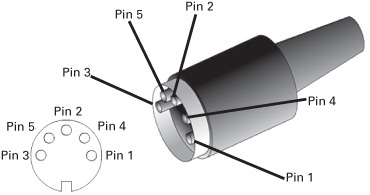
\includegraphics[scale=0.8]{Imagens/MIDI_connector.jpg}
            	\caption[Conector MIDI]{Conector MIDI}
            	\label{fig:MIDI_connector}
            \end{figure}

            O conector MIDI, semelhante ao apresentado na figura ~\ref{fig:MIDI_connector}, apresenta 5 pinos distintos. Entretanto, como já mencionado, MIDI envia informações utilizando um protocolo de transmissão serial. Desta forma, apenas um pino é realmente utilizado para o envio de informações. A tabela ~\ref{table:MIDI_pins} descreve cada pino do conector e sua respectiva função.

            \begin{center}
                \tablefirsthead{%
                  \hline
                  \rowcolor{darkRed} \textcolor{white}{\textbf{Pino}} & \textcolor{white}{\textbf{Descrição}} \\
                  \hline}
                \tablehead{%
                  \hline
                  \multicolumn{2}{|l|}{\small\sl continuação da página anterior} \\
                  \hline
                  \rowcolor{darkRed} \textcolor{white}{\textbf{Pino}} & \textcolor{white}{\textbf{Descrição}} \\
                  \hline}
                \tabletail{%
                  \hline
                  \multicolumn{2}{|r|}{\small\sl continua na próxima página} \\
                  \hline}
                \tablelasttail{\hline}
                \bottomcaption{Pinos em um conector MIDI
                \label{table:MIDI_pins}}
                %
                \begin{supertabular}{| C{0.8cm} | C{14.3cm} |}
                    \rowcolor{lightRed} 1 &  Não é utilizado. Na maioria dos cabos MIDI, este pino não está conectado a nenhum fio. \\
                    \rowcolor{white}    2 &  Este é utilizado para proteção elétrica (~\sigla{GND}{Ground}). Esta proteção impede que a transmissão apresente sinais elétricos indesejados. \\
                    \rowcolor{lightRed} 3 &  Como o Pino 1, este também não é utilizado, e na maioria dos cabos MIDI, também não está conectado a nenhum fio. \\
                    \rowcolor{white}    4 &  Este é o único receptor de dados MIDI. As informações através deste cabo fluem em uma única direção. \\
                    \rowcolor{lightRed} 5 &  Este é o único transmissor de dados MIDI e, assim como no pino 4, as informações também fluem unidirecionalmente. \\
                \end{supertabular}
            \end{center}

            Além do conector, outro hardware importante, que vale a pena ser ressaltado, é a versão fêmea do cabo MIDI. Controladores MIDI, como o desenvolvido neste projeto, apresentam normalmente 2 ou 3 destes conectores, rotulados como \textbf{In}, \textbf{Out} e \textbf{~\sigla{Thru}{Through}} (veja a figura ~\ref{fig:MIDI_connector_Female}). O conjunto destes conectores é chamado de \textbf{porta MIDI} e cada uma deles será explicado com mais detalhes a seguir.

            \begin{figure}[H]
            	\centering
            	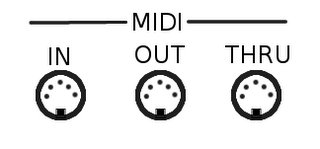
\includegraphics[scale=0.8]{Imagens/midi_in_out_thru.png}
            	\caption[Conectores fêmeas MIDI]{Conectores fêmeas MIDI}
            	\label{fig:MIDI_connector_Female}
            \end{figure}

            \begin{itemize}
                \item MIDI IN: Através deste conector são recebidas as mensagens MIDI de um determinado dispositivo ou software MIDI. Estas mensagens podem então ser processadas e, caso desejado, enviadas para outro dispositivo através do conector MIDI Thru.

                \item MIDI OUT: Através deste conector são transmitidas as mensagens MIDI que são geradas em um software ou dispositivo MIDI. Esta saída não envia informação de áudio, mas sim simples mensagens MIDI que são interpretadas por um conector MIDI In de um outro dispositivo. Tais mensagens são códigos digitais que representam o que e como músicas e eventos são tocados em um determinado instrumento.

                \item MIDI THRU: envia uma réplica do sinal recebido na porta In para o componente ligado a ele, seja em cadeia ou somente os dois, desde que sejam componentes MIDI.
            \end{itemize}

        \subsection{Formatos de distribuição}

            Como já dito no início deste capítulo, existe um formato de arquivo padrão para MIDI, o SMF. Este tipo de arquivo armazena todas as informações necessárias para reproduzir todos os parâmetros suportados pelo protocolo. Além disso, ele também adiciona o que chamamos de \textit{time stamp} em cada evento, para que o software MIDI, ou até mesmo o usuário final, saiba o momento correto de realizar cada um destes.

            MIDI tem a vantagem de ser compacto, uma vez que o som tocado por determinado instrumento não é gravado, mas sim apenas as informações de cada evento. Devido a este fato, arquivos MIDI apresentam um tamanho cerca de 300 vezes menor do que um arquivo de música atual (MP3). Entretanto, esse valor pode ser muito maior se compararmos com formatos descompactados de músicas.

            O fato de MIDI não gravar som, entretanto, pode também ser uma desvantagem. Quando o som de um determinado instrumento é gravado, o usuário tem total controle sobre o resultado final, enquanto com MIDI, este mesmo resultado depende do dispositivo ou software que será utilizado para reproduzir este mesmo som.

        \subsection{Canais MIDI}

            Quando trabalhamos com música, muitas vezes desejamos que diversos instrumentos participem da mesma composição. Com MIDI, podemos incluir instruções para cada um deles através dos chamados \textbf{canais MIDI}.

            Pense em um canal MIDI como um canal de televisão (veja a figura ~\ref{fig:midi-channels}). Um determinado instrumento conecta-se apenas a um único canal, assim como um usuário o faz em sua televisão. Isso não significa que os outros canais não estão disponíveis, mas sim que o conteúdo disponível (no nosso caso, a mensagem MIDI) foi filtrado para processar apenas o relevante para aquele canal.

            \begin{figure}[H]
            	\centering
            	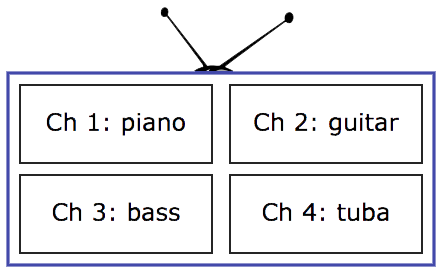
\includegraphics[scale=0.6]{Imagens/midi-channels.png}
            	\caption[Exemplo de canais MIDI]{Exemplo de canais MIDI ~\cite{Gibson2013}}
            	\label{fig:midi-channels}
            \end{figure}

            Cada porta MIDI suporta até 16 canais simultâneos. Em outras palavras, um usuário pode escolher um determinado canal para transmitir as mensagens MIDI ou possuir até 16 instrumentos conectados simultaneamente, cada um realizando diferentes eventos.

    \section{Mensagens MIDI}

        Agora que já explicamos o básico sobre o protocolo MIDI, é necessário estudarmos como podemos transmitir informações através de dispositivos. Essas informações são as chamadas \textbf{mensagens MIDI}.

        O conteúdo de uma mensagem MIDI é bastante simples. Todas elas apresentam um componente chamado de \textit{status byte}. Este componente é acompanhado por um valor que é definido por um ou mais \textit{bytes} de dados.

        Durante essa seção, os seguintes tópicos serão abordados:

        \begin{itemize}
                \item A estrutura de uma mensagem MIDI.

                \item Diferenças entre os tipos de mensagens MIDI.

                \item O que essas mensagens contêm e o que seus valores representam.

                \item Como MIDI atribui nomes e números de notas para cada evento.

                \item Como as mensagens MIDI transmitem e armazenam informações sobre a performance, e então as reproduzem no tempo correto.
        \end{itemize}

        \subsection{Mensagens de estado e de dados}

            Como já visto na seção anterior, cada \textit{byte} em uma mensagem MIDI contém 10 \textit{bits}. Destes, 8 são utilizados para a transmissão de informações. Desta forma, cada mensagem pode conter um valor entre 0 e 255. Tais mensagens são divididas em duas categorias: \textit{Estado} e \textit{Dados} (veja a figura ~\ref{fig:Status_and_Data_Bytes}).

            \begin{figure}[H]
            	\centering
            	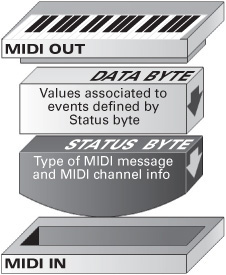
\includegraphics[scale=0.8]{Imagens/Status_and_Data_Bytes.jpg}
            	\caption[Byte de estado e de dados]{Byte de estado e de dados ~\cite{Guerin}}
            	\label{fig:Status_and_Data_Bytes}
            \end{figure}

            \begin{itemize}
                \item A porção referente ao \textit{byte} de estado serve para identificar o tipo de informação que está sendo enviada. Ela informa ao dispositivo receptor a qual canal MIDI determinado evento pertence e o que este evento é. Um evento pode ser, por exemplo, um Note On ou um Note Off. Outros eventos serão explicados no decorrer do projeto.

                \item A porção referente ao \textit{byte} de dados informa ao dispositivo receptor o valor que está associado ao evento determinado na outra porção da mensagem MIDI. Por exemplo, se o usuário decidir tocar um \textit{Dó} mediano com uma força também mediana, o \textit{byte} de estado irá enviar um evento "Note On", enquanto o \textit{byte} de dados irá passar o valor correspondente à essa nota e à velocidade que esta foi tocada. No nosso exemplo, a nota C4 tem o valor correspondente a 60 (veja a tabela ~\ref{table:MIDI_notes}) e a velocidade de aproximadamente 64.
            \end{itemize}

            Os valores utilizados pelo \textit{byte} de estado variam entre 128 e 255 (1000 0000 a 1111 1111 em números binários), enquanto para o \textit{byte} de dados estes variam entre 0 a 127 (0000 0000 a 0111 1111 em números binários). É fácil perceber que, para um dispositivo MIDI reconhecer qual o tipo de mensagem que se está sendo transmitida, basta verificar o \sigla{MSB}{Most Significant Bit} (\textit{Bit} mais significativo, do inglês). Se este valor for 1, trata-se de um \textit{byte} de estado. Caso contrário, de um \textit{byte} de dados. Simples assim.

            Digamos que um dispositivo MIDI receba três valores: 175, 43 e 125. Ele saberá que 175 é um \textit{byte} de estado, enquanto os outros dois valores são os \textit{bytes} de dados que estão acompanhando o \textit{byte} de estado. Caso este dispositivo receba outros valores, digamos: 200, 220 e 90. Ele saberá que os dois primeiros valores são \textit{bytes} de estados, enquanto o último é um \textit{byte} de dados que acompanha apenas o último \textit{byte} de estado, não ambos.

            Mensagens MIDI são normalmente representadas em um dos três mais comuns formatos digitais: decimais; binários; e hexadecimais. Explicar a conversão entre estes formatos (e os formatos em si) jazem fora do escopo deste projeto, mas podem ser consultados no livro \textit{MIDI Power!}~\cite{Guerin}.
            
            

    \section{Microcontroladores e Arduino}



        \subsection{Microcontroladores}



        \subsection{Arduino}


    %%
%% Desenvolvimento.tex
%% Projeto Oficinas de Integração 3
%% Created by Leonardo Winter Pereira and Lucas Zimmermann Cordeiro on 10.03.2016
%% Copyright (C). All rights reserved
%%

\chapter{Desenvolvimento}
\label{chap:desenvolvimento}



    \section{Hardware}



    \section{Estação Base Principal}



        \subsection{Interface}



        \subsection{Lógica}



    \section{Estação Base Secundária}



        \subsection{Interface}



        \subsection{Lógica}



    \section{Comunicação entre Hardware e Software}

        Nesta seção discutiremos como foi realizada a comunicação entre o Hardware e o Software do Dalle Pad.

    \section{Projeto Mecânico - Invólucro}

        
    %%
%% Resultados.tex
%% Projeto Oficinas de Integração 3
%% Created by Leonardo Winter Pereira and Lucas Zimmermann Cordeiro on 10.03.2016
%% Copyright (C). All rights reserved
%%

\chapter{Resultados e Discussões}
\label{chap:resultados} 


    %%
%% Conclusao.tex
%% Projeto Oficinas de Integração 3
%% Created by Leonardo Winter Pereira and Lucas Zimmermann Cordeiro on 10.03.2016
%% Copyright (C). All rights reserved
%%

\chapter{Considerações Finais}
\label{chap:consideracoesFinais} 



    \section{Sugestões para trabalhos futuros}
    
    

    %---------- Referências ----------
    \bibliography{reflatex} % Geração automática das referências a partir do arquivo reflatex.bib

    \apendice
    %%
%% Apendice.tex
%% Projeto Oficinas de Integração 3
%% Created by Leonardo Winter Pereira and Lucas Zimmermann Cordeiro on 10.03.2016
%% Copyright (C). All rights reserved
%%

%% Apêndice é um texto ou documento elaborado pelo autor do TC, ou seja,
%% se foi necessário você criar uma entrevista, um relatório, ou qualquer
%% documento com o escopo de complementar sua argumentação


\chapter{Nome do Apêndice}

    \section{Notas musicais em MIDI}
    
        O estudo da música em si está fora do escopo deste projeto. Entretanto, é imprescindível entender o que é uma oitava. Segue uma breve definição: \epigraph{Uma oitava é o intervalo entre uma nota musical e outra com a metade ou o dobro de sua frequência.}{~\cite{WikipediaOitava}}
        
        Dizer que uma nota está uma oitava acima significa dizer que a nota é a mesma, porém ela está em uma região mais aguda do instrumento.
    
        \definecolor{darkRed}{rgb}{0.607843137254902, 0.1764705882352941, 0.1215686274509804}
        \definecolor{lightRed}{rgb}{0.9568627450980392, 0.803921568627451, 0.7843137254901961}
        
        \begin{table}[H]
            \centering
            \begin{tabular}{| c | c | c | c | c | c | c | c | c | c | c | c | c |}
                \hline
                %\rowcolor{darkRed} \textcolor{white}{\textbf{Oitava}} & \textcolor{white}{\textbf{Número referente a nota}} \\
                \rowcolor{darkRed} \textcolor{white}{\textbf{Oitava}} & \textcolor{white}{\textbf{C}} & \textcolor{white}{\textbf{C\#}} & \textcolor{white}{\textbf{D}} & \textcolor{white}{\textbf{D\#}} & \textcolor{white}{\textbf{E}} & \textcolor{white}{\textbf{F}} & \textcolor{white}{\textbf{F\#}} & \textcolor{white}{\textbf{G}} & \textcolor{white}{\textbf{G\#}} & \textcolor{white}{\textbf{A}} & \textcolor{white}{\textbf{A\#}} & \textcolor{white}{\textbf{B}} \\
                \hline
                \rowcolor{lightRed} \textbf{-1} &  0   & 1   & 2   & 3   & 4   & 5   & 6   & 7   & 8   & 9   & 10 & 11 \\
                \hline
                \rowcolor{white}     \textbf{0} &  12  & 13  & 14  & 15  & 16  & 17  & 18  & 19  & 20  & 21  & 22 & 23 \\
                \hline
                \rowcolor{lightRed}  \textbf{1} &  24  & 25  & 26  & 27  & 28  & 29  & 30  & 31  & 32  & 33  & 34 & 35 \\
                \hline
                \rowcolor{white}     \textbf{2} &  36  & 37  & 38  & 39  & 40  & 41  & 42  & 43  & 44  & 45  & 46 & 47 \\
                \hline
                \rowcolor{lightRed}  \textbf{3} &  48  & 49  & 50  & 51  & 52  & 53  & 54  & 55  & 56  & 57  & 58 & 59 \\
                \hline
                \rowcolor{white}     \textbf{4} &  60  & 61  & 62  & 63  & 64  & 65  & 66  & 67  & 68  & 69  & 70 & 71 \\
                \hline
                \rowcolor{lightRed}  \textbf{5} &  72  & 73  & 74  & 75  & 76  & 77  & 78  & 79  & 80  & 81  & 82 & 83 \\
                \hline
                \rowcolor{white}     \textbf{6} &  84  & 85  & 86  & 87  & 88  & 89  & 90  & 91  & 92  & 93  & 94 & 95 \\
                \hline
                \rowcolor{lightRed}  \textbf{7} &  96  & 97  & 98  & 99  & 100 & 101 & 102 & 103 & 104 & 105 & 106 & 107 \\
                \hline
                \rowcolor{white}     \textbf{8} &  108 & 109 & 110 & 111 & 112 & 113 & 114 & 115 & 116 & 117 & 118 & 119 \\
                \hline
                \rowcolor{lightRed}  \textbf{9} &  120 & 121 & 122 & 123 & 124 & 125 & 126 & 127 &     &     &     &     \\
                \hline
            \end{tabular}
            \caption{Notas musicais em MIDI}
            \label{table:MIDI_notes}
        \end{table}

%% ---------------- 4 -------------------
%% O Gerenciamento da Integração do Projeto descreve os processos necessários para assegurar que os diversos elementos do projeto sejam adequadamente coordenados.
%% A integração envolve tomada de decisão e escolhas diretamente ligadas aos objetivos do projeto e aos processos das etapas de desenvolvimento e execução do plano do projeto, assim como ao processo de controle de alterações.
%% O gerenciamento da integração é composto pelos processos: desenvolvimento do plano do projeto, execução do plano do projeto e controle integrado de mudanças
%\chapter{Gerenciamento de Integração do Projeto}



    %% ---------------- 4.1 -------------------
%    \section{Termo de Abertura do Projeto}

%    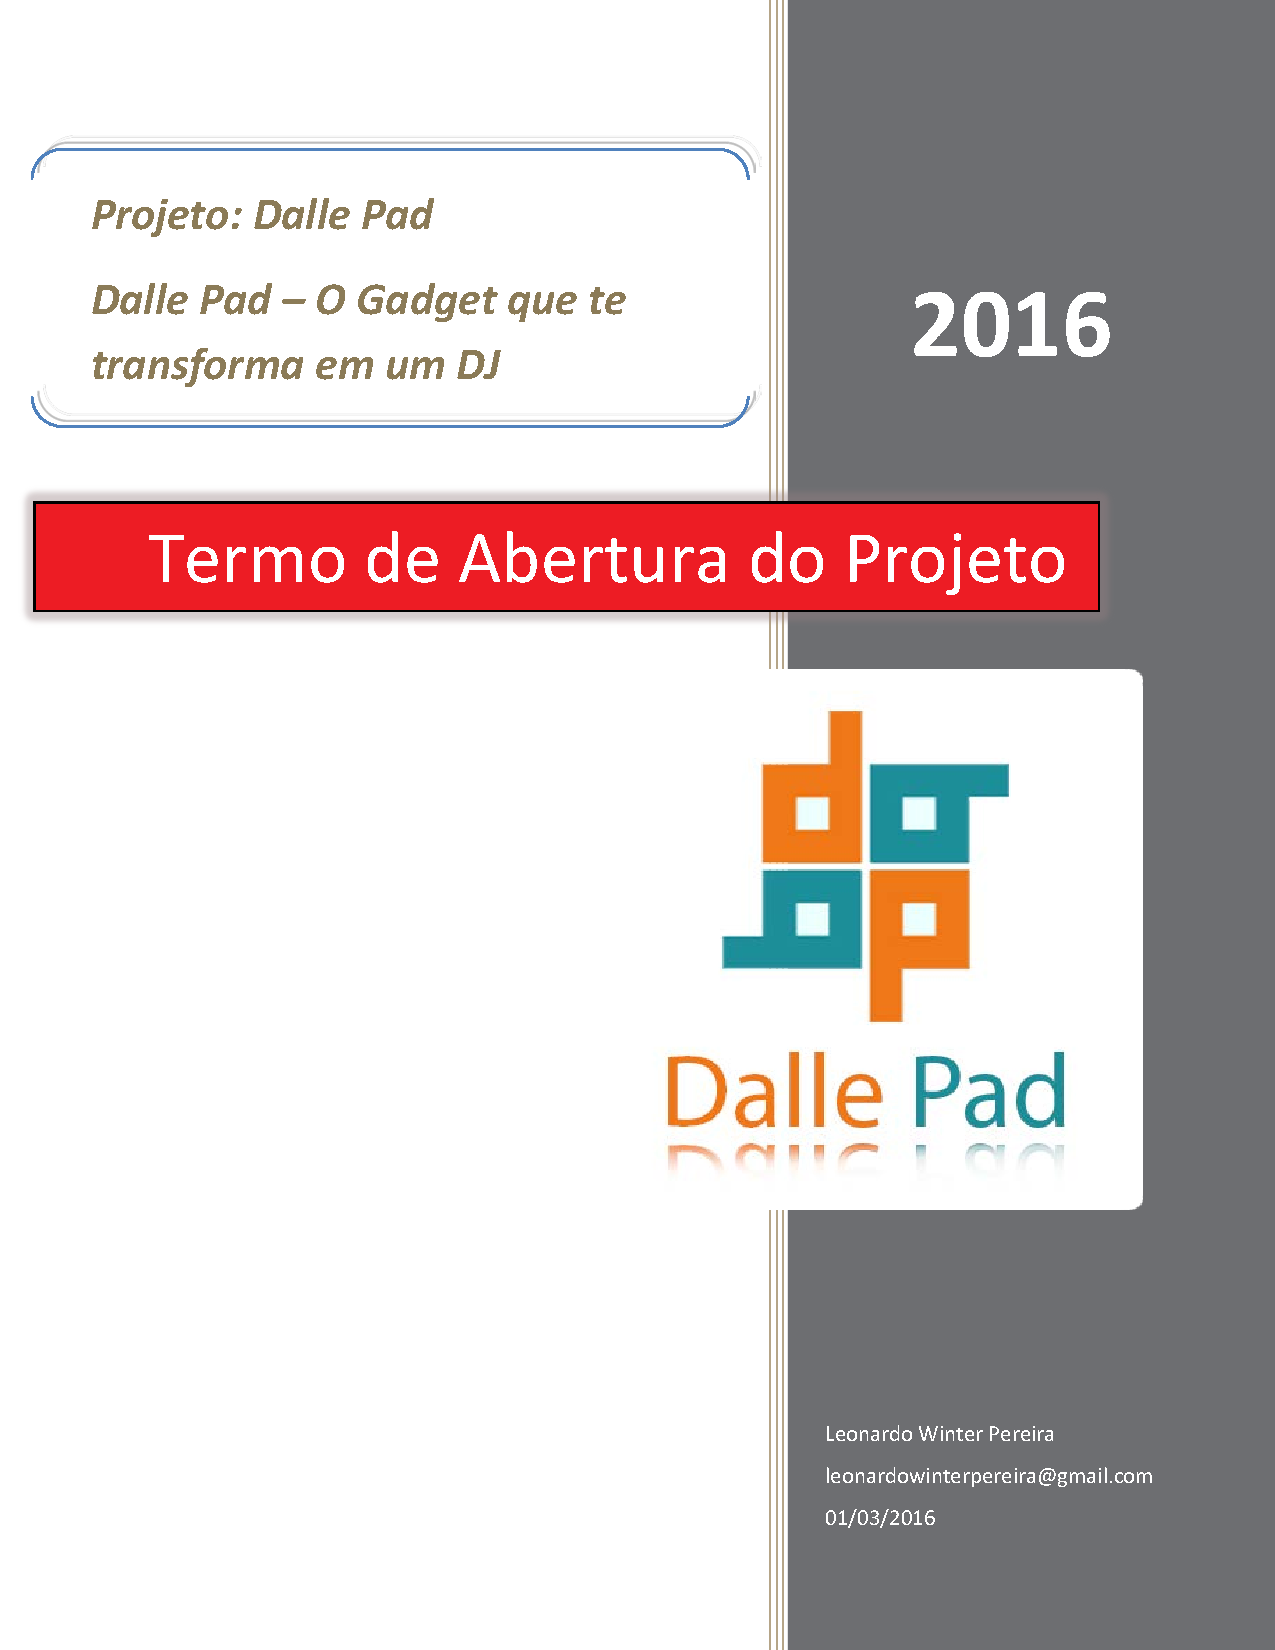
\includepdf[pages={-}]{Documentos/Termo_de_Abertura_de_Projeto.pdf}

    %% ---------------- 4.2 -------------------
%    \section{Declaração do Escopo Preliminar do Projeto}



    %% ---------------- 4.3 -------------------
%    \section{Plano de Gerenciamento do Projeto}

%    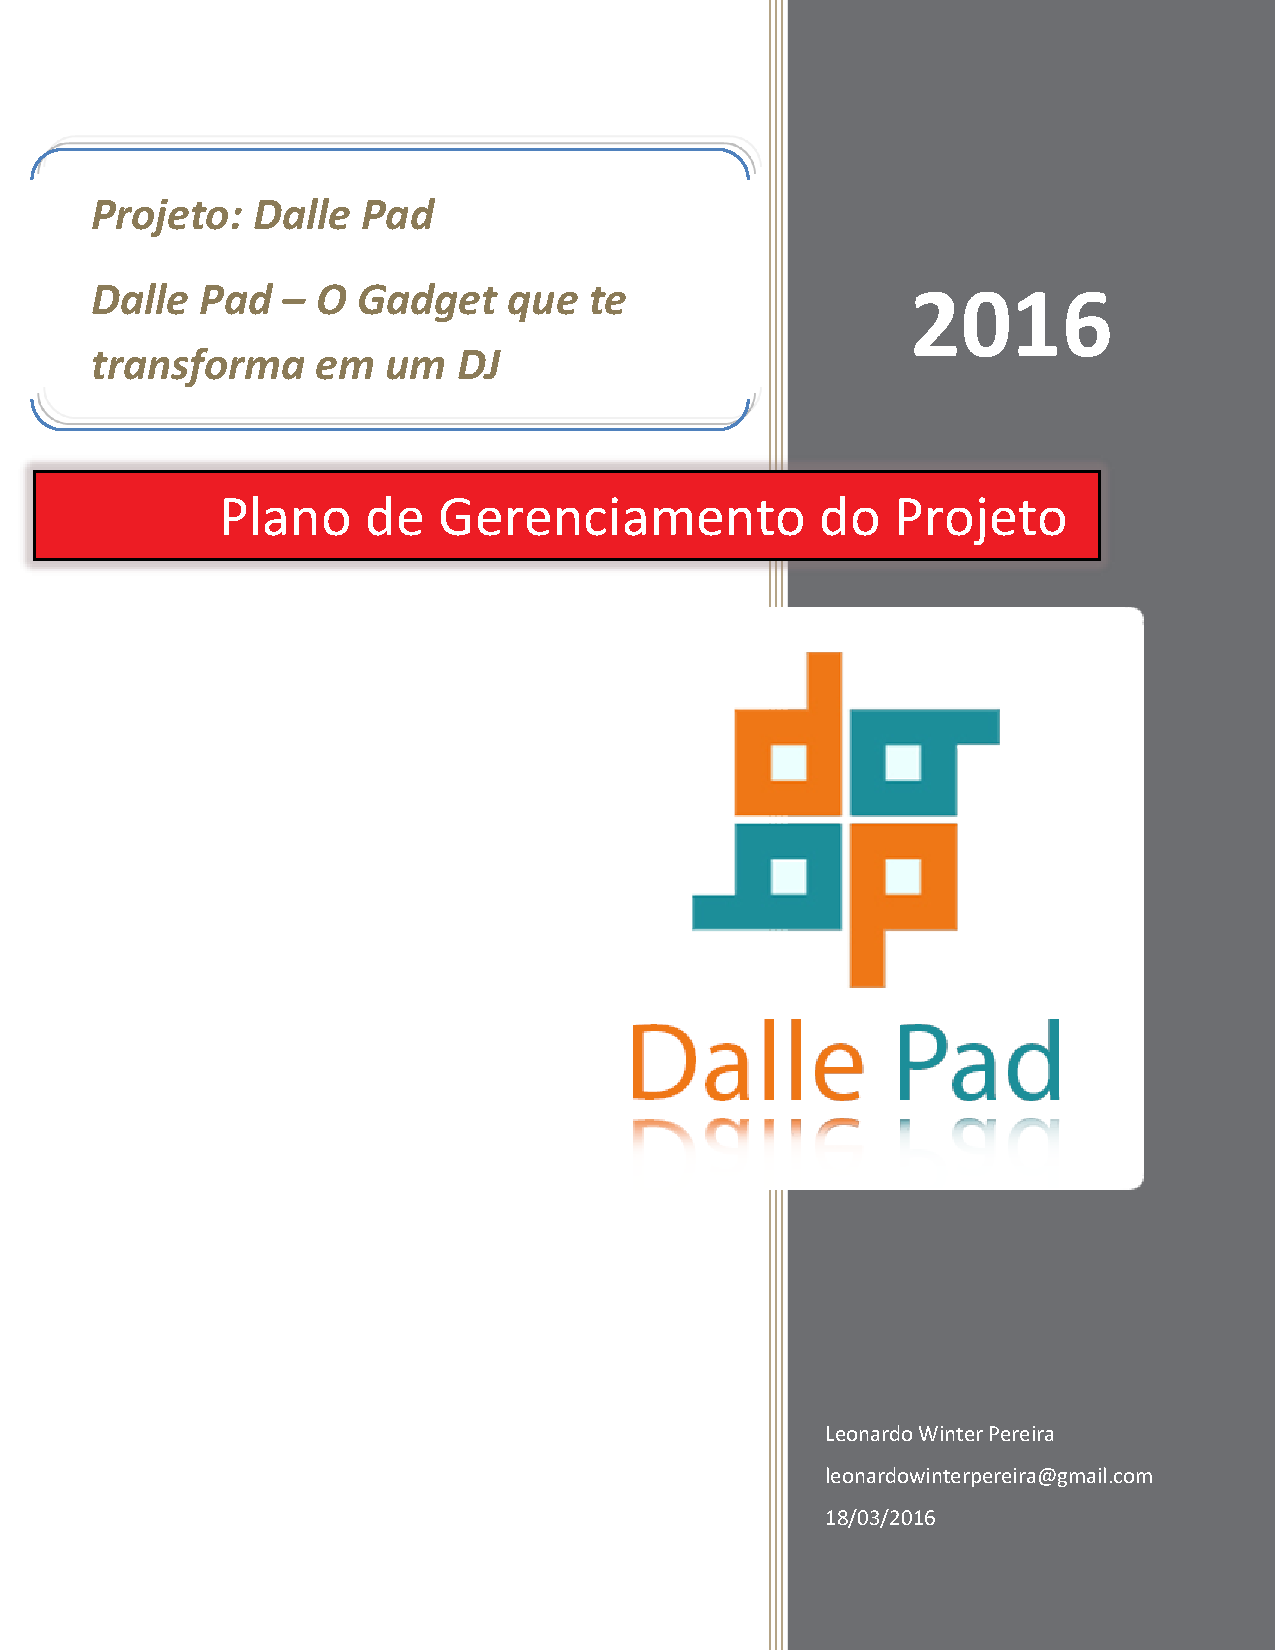
\includepdf[pages={-}]{Documentos/Plano_de_Projeto.pdf}

%% ---------------- 5 -------------------
%% O Gerenciamento do Escopo do Projeto descreve os processos necessários para assegurar que o projeto contemple todo o trabalho requerido, e nada mais que o trabalho requerido, para completar o projeto com sucesso.
%% A preocupação fundamental é definir e controlar o que está ou não, incluído no projeto.
%% Ele é composto pelos processos: iniciação, planejamento do escopo, detalhamento do escopo, verificação do escopo e controle de mudanças do escopo.
%\chapter{Gerenciamento de Escopo do Projeto}



    %% ---------------- 5.1 -------------------
%    \section{Planejamento do Escopo}



    %% ---------------- 5.2 -------------------
%    \section{Definição do Escopo}



    %% ---------------- 5.3 -------------------
%    \section{Estrutura Analítica do Projeto}



%% ---------------- 6 -------------------
%% O Gerenciamento do Tempo do Projeto descreve os processos necessários para assegurar que o projeto termine dentro do prazo previsto.
%% Ele é composto pelos processos: definição das atividades, sequenciamento das atividades, estimativa da duração das atividades, desenvolvimento do cronograma e controle do cronograma.
%\chapter{Gerenciamento do Tempo do Projeto}



    %% ---------------- 6.1 -------------------
%    \section{Definição da Atividade}



    %% ---------------- 6.2 -------------------
%    \section{Sequenciamento de Atividades}



    %% ---------------- 6.3 -------------------
%    \section{Estimativa de recursos de atividade}



    %% ---------------- 6.4 -------------------
%    \section{Estimativa de duração de atividade}



    %% ---------------- 6.5 -------------------
%    \section{Desenvolvimento do Cronograma}



%% ---------------- 7 -------------------
%% O Gerenciamento do Custo do Projeto descreve os processos necessários para assegurar que o projeto termine dentro do orçamento aprovado.
%% Ele é composto pelos processos: planejamento dos recursos, estimativa dos custos, orçamento dos custos e controle dos custos.
%% No projeto, várias atividades afetam os custos do projeto e desta forma, o planejamento e controle dos custos são fundamentais.
%\chapter{Gerenciamento do Custo do Projeto}



    %% ---------------- 7.1 -------------------
%    \section{Estimativa de custos}



    %% ---------------- 7.2 -------------------
%    \section{Orçamentação}



%% ---------------- 8 -------------------
%% O Gerenciamento da Qualidade do Projeto descreve os processos necessários para assegurar que as necessidades que originaram o desenvolvimento do projeto serão satisfeitas.
%% O projeto tem qualidade quando é concluído de acordo com os requisitos, especificações (o projeto deve produzir o que foi definido) e adequação ao uso (deve satisfazer às reais necessidades dos clientes).
%% O gerenciamento da qualidade é composto pelos processos: planejamento da qualidade, garantia da qualidade e controle da qualidade.
%\chapter{Gerenciamento da Qualidade do Projeto}



    %% ---------------- 8.1 -------------------
%    \section{Planejamento da qualidade}



%% ---------------- 9 -------------------
%% O Gerenciamento dos Recursos Humanos do Projeto descreve os processos necessários para proporcionar a melhor utilização das pessoas envolvidas no projeto. Embora seja uma área de conhecimento, na maioria das vezes, complexa e subjetiva exige constante pesquisa, sensibilidade e muita vivência do dia-a-dia para saber lidar com o ser humano.
%% É composta pelos processos: planejamento organizacional, montagem da equipe e desenvolvimento da equipe.
%\chapter{Gerenciamento de Recursos Humanos do Projeto}



    %% ---------------- 9.1 -------------------
%    \section{Planejamento de recursos humanos}



%% ---------------- 10 -------------------
%% O Gerenciamento das Comunicações do Projeto descreve os processos necessários para assegurar a geração, captura, distribuição, armazenamento e pronta apresentação das informações do projeto para que sejam feitas de forma adequada e no tempo certo.
%% A gestão da comunicação é frequentemente ignorada pelos gerentes de projeto, no entanto nos projetos concluídos com sucesso o gerente gasta 90% do seu tempo envolvido com algum tipo de comunicação (formal, informal, verbal, escrita).
%% Este gerenciamento é composto pelos processos: planejamento das comunicações, distribuição das informações, relato de desempenho e encerramento administrativo
%\chapter{Gerenciamento de Comunicação do Projeto}



    %% ---------------- 10.1 -------------------
%    \section{Planejamento das comunicações}



%% ---------------- 11 -------------------
%% O Gerenciamento dos Riscos do Projeto descreve os processos que dizem respeito à identificação, análise e resposta aos riscos do projeto.
%% A prática deste gerenciamento não é ainda muito comum na maioria das organizações e alguns autores citam que gerenciar projetos é gerenciar riscos.
%% O gerenciamento de riscos é muito importante para o sucesso do projeto e é composto pelos seguintes processos: Planejamento da Gerência de Risco, identificação dos riscos, análise qualitativa de riscos, análise quantitativa de riscos, desenvolvimento das respostas aos riscos e controle e monitoração de riscos.
%\chapter{Gerenciamento do Risco do Projeto}



    %% ---------------- 11.1 -------------------
%    \section{Planejamento do gerenciamento de riscos}



    %% ---------------- 11.2 -------------------
%    \section{Identificação de riscos}



    %% ---------------- 11.3 -------------------
%    \section{Análise Qualitativa de riscos}



    %% ---------------- 11.4 -------------------
%    \section{Planejamento de respostas a riscos}



%% ---------------- 12 -------------------
%% O Gerenciamento das Aquisições do Projeto descreve os processos necessários para a aquisição de mercadorias e serviços fora da organização que desenvolve o projeto.
%% Este gerenciamento é discutido do ponto de vista do comprador na relação comprador-fornecedor.
%% Ele é composto pelos processos: planejamento das aquisições, preparação das aquisições, obtenção de propostas, seleção de fornecedores, administração dos contratos e encerramento do contrato.
%\chapter{Gerenciamento das Aquisições do Projeto}



    %% ---------------- 12.1 -------------------
%    \section{Planejar compras e aquisições}



    %% ---------------- 12.2 -------------------
%    \section{Planejar contratações}



%% Atas de Reunião são importantes pois definem exatamente o que foi / será discutido em cada reunião da Equipe Dalle Pad!
%\chapter{Atas de Reunião}




    \anexo
    %%
%% Anexos.tex
%% Projeto Oficinas de Integração 3
%% Created by Leonardo Winter Pereira and Lucas Zimmermann Cordeiro on 10.03.2016
%% Copyright (C). All rights reserved
%%

%% Anexo é um texto ou documento não elaborado pelo autor
%% do Trabalho Científico (TC) (monografia, tese, etc.)

\chapter{Datasheets}
\label{chap:anexosA}

    Este capítulo compreende todos os \textit{datasheets} de terceiros utilizados durante o desenvolver do projeto.

    É importante ressaltar que os componentes desenvolvidos pela própria equipe, sistemas eletrônicos e códigos estão todos relatados no capítulo anterior.

    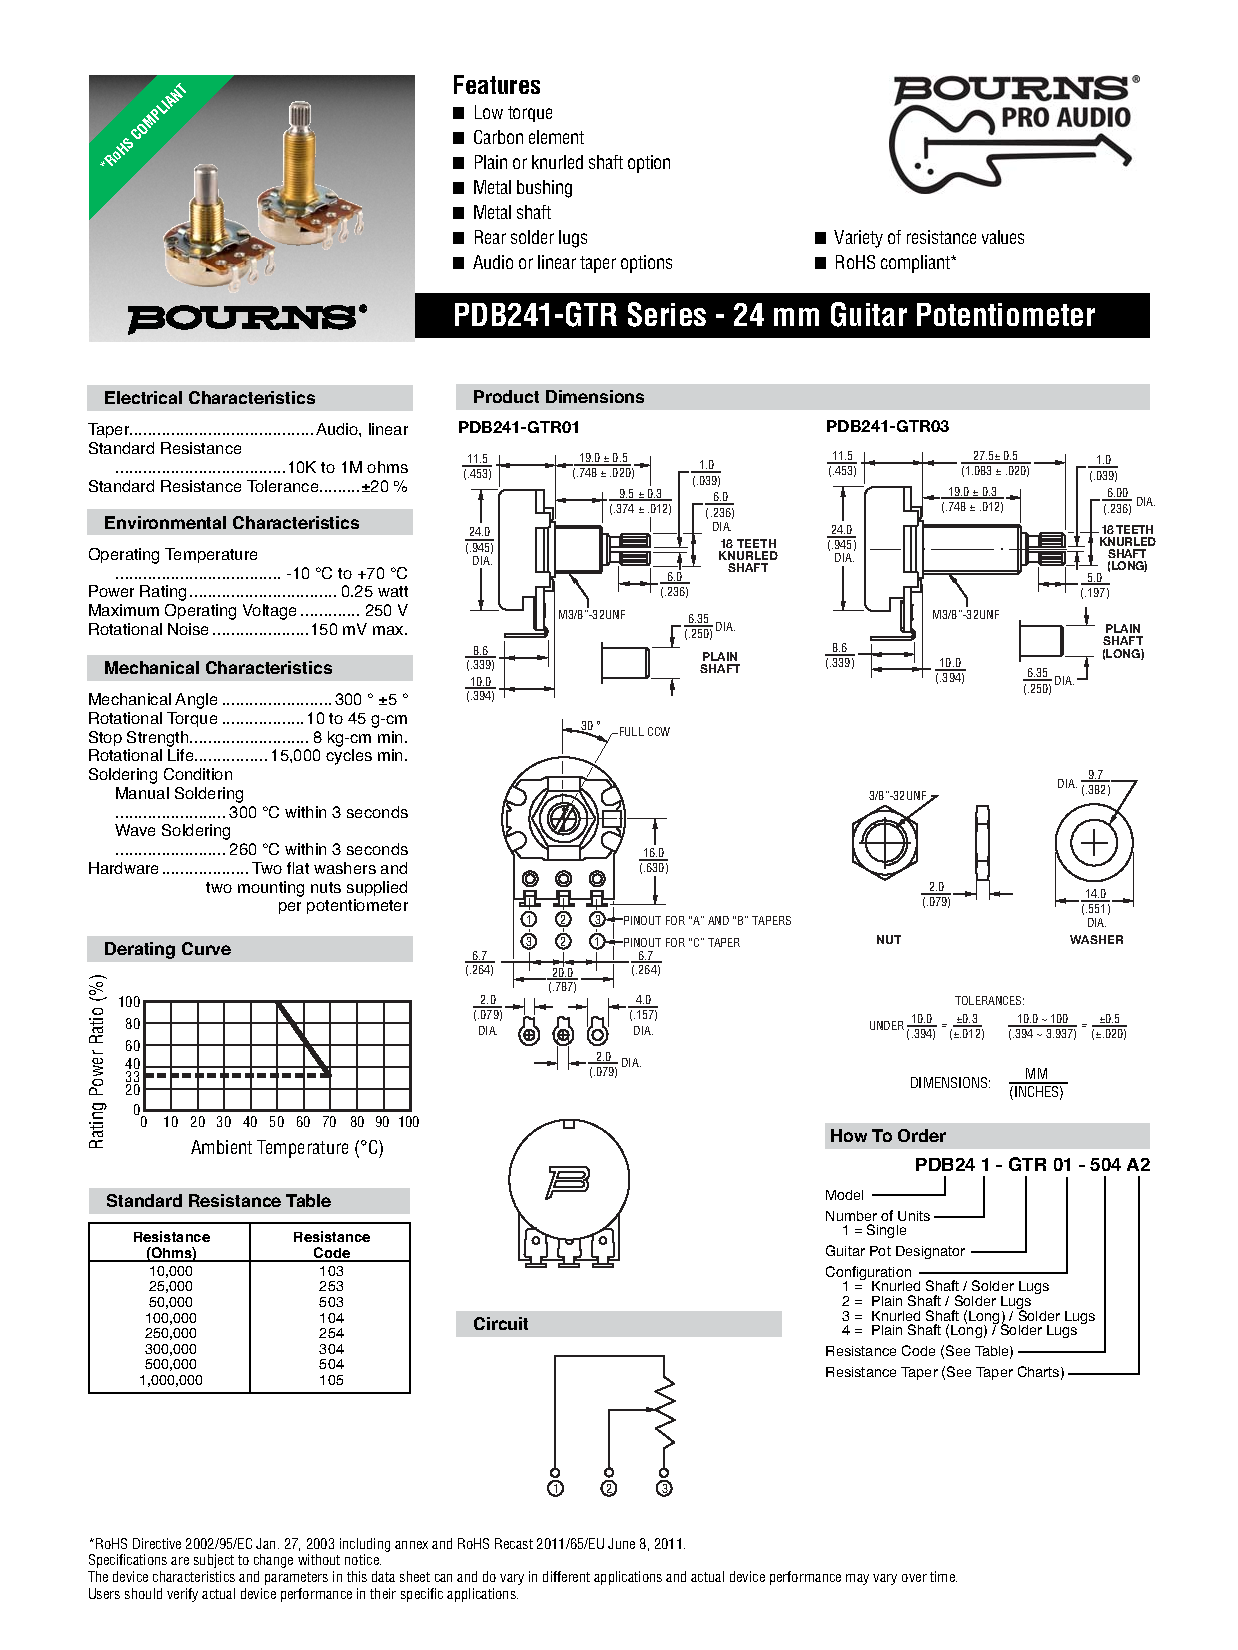
\includepdf[scale={0.8}, pages={1}, pagecommand=\section{Potenciômetro rotativo}]{../Datasheets/rotary_potentiometer.pdf}

    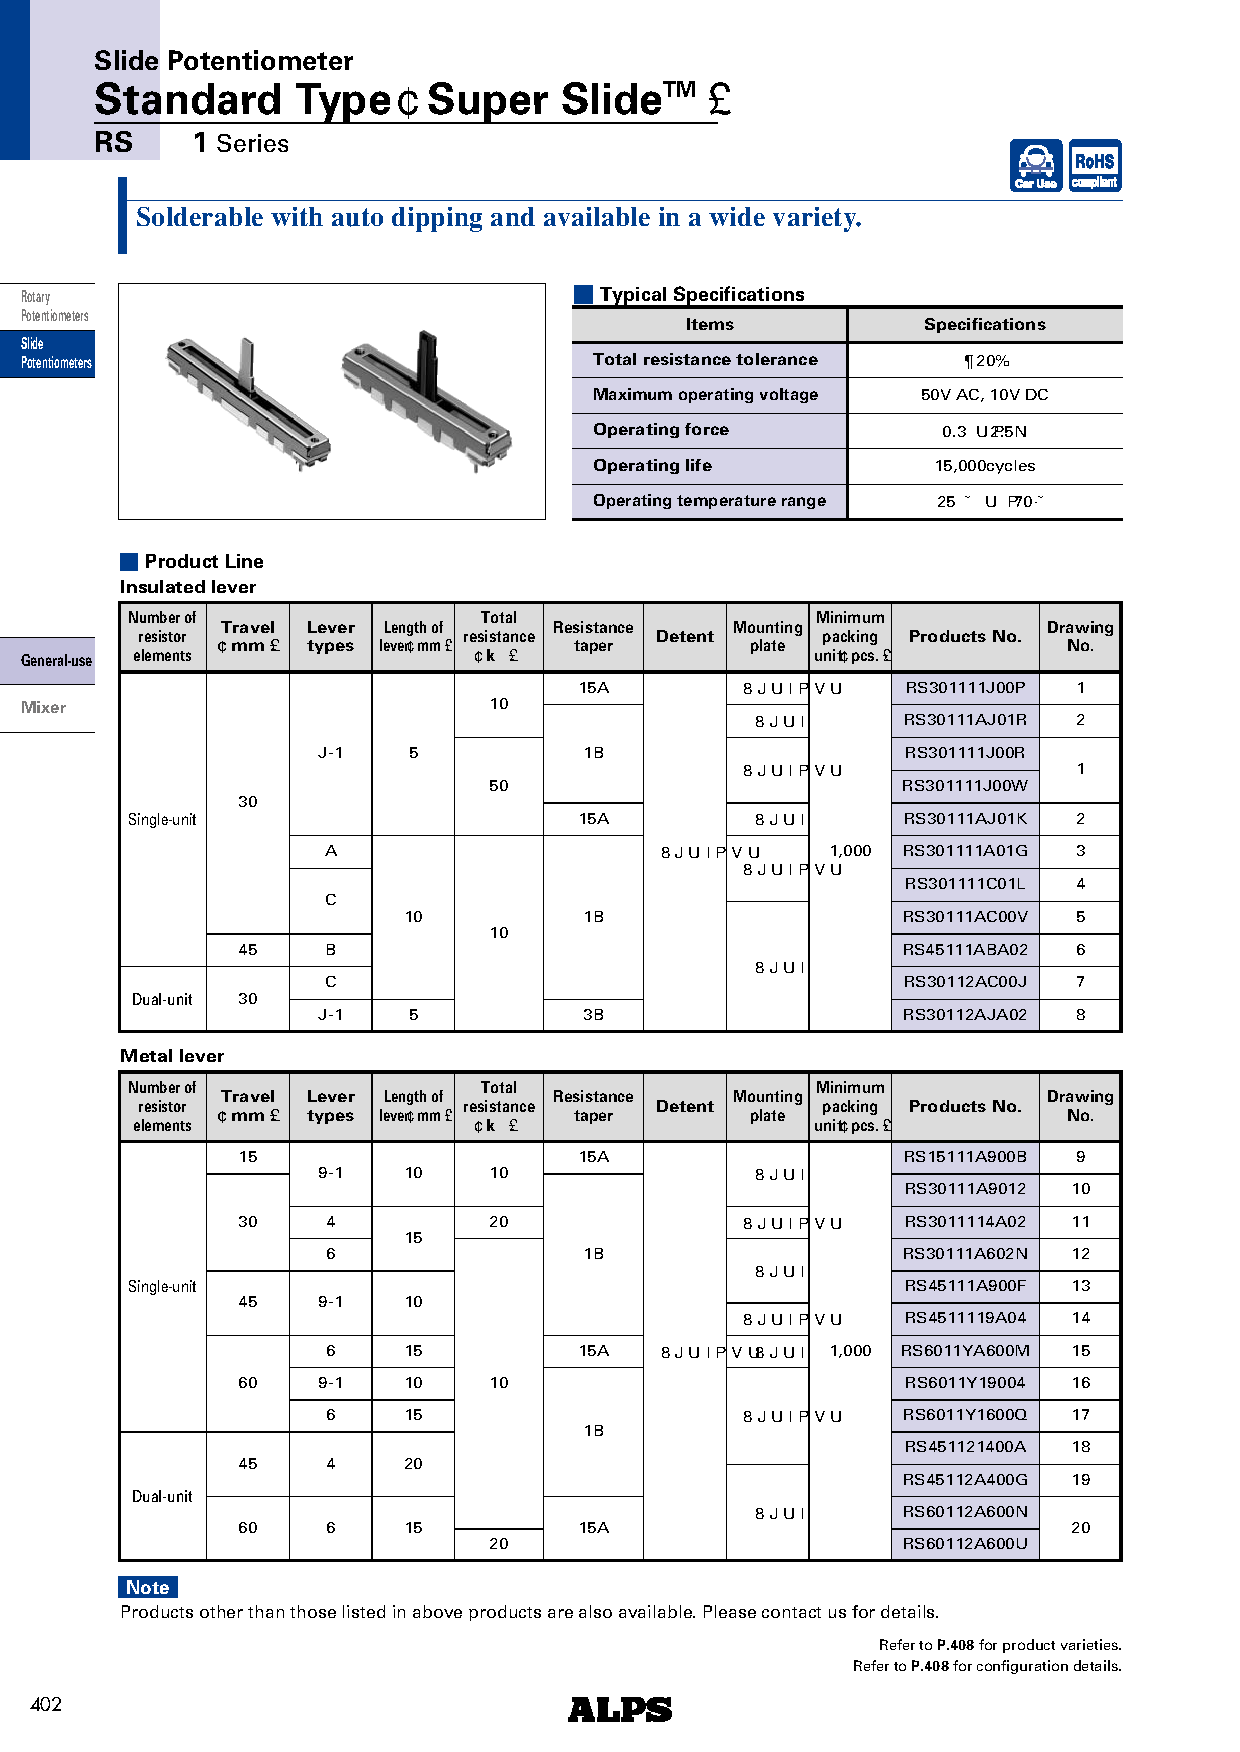
\includepdf[scale={0.7}, pages={1}, pagecommand=\section{Potenciômetro linear}]{../Datasheets/linear_potentiometer_b10k.pdf}
    \includepdf[scale={0.8}, pages={6}, pagecommand={}]{../Datasheets/linear_potentiometer_b10k.pdf}
    \includepdf[scale={0.8}, pages={9}, pagecommand={}]{../Datasheets/linear_potentiometer_b10k.pdf} 

\end{document} 